\chapter{Facebook Privacy}
\label{chp:defaultprivacysettings} 

In this chapter we are going to look into was kind of privacy settings that exist on Facebook and the history of Facebook's privacy settings. We will also look at and map how the default privacy settings has evolved over time. In addition to this we will look at some of the features introduced by Facebook over the years, and how these features have effected the privacy on Facebook. Finally we will review some of Mark Zuckerberg's  thoughts and comments in regard to Facebook privacy. 


\section{Privacy on Facebook}\label{sec:privacy_on_facebook}

%-dra inn undersøkelse 
%-hva slags type settings som finnes? 

\begin{figure}[h!]
\centering
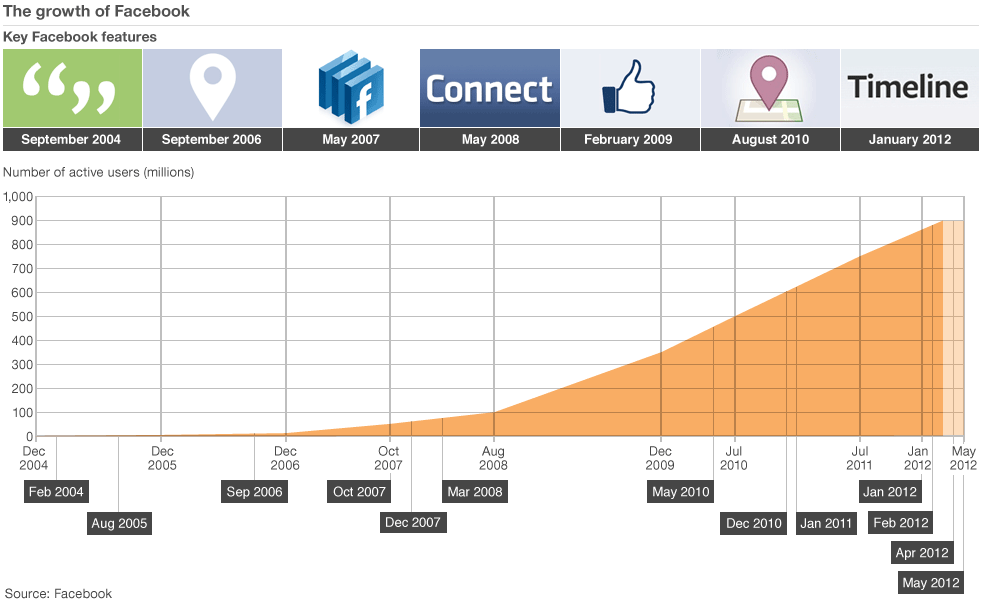
\includegraphics[width=0.8\textwidth]{gowth_of_facebook.png}
\caption[The development of Facebook users and introduction of new features]{\textbf{The development of Facebook users and introduction of new features.} The orange field in the graph shows the increasing number of Facebook users over the years. Key Facebook features are shown over the graph according to when they were introduced \cite{BBCFacebookGrowth}.} 
\label{fig:growth_of_facebook}
\end{figure}

There is no doubt that Facebook has had a remarkable development, both when it comes to number of active users and the development of new features, as shown in \fref{fig:growth_of_facebook}. Along with new users and new features, there has also been made changes to what kind of privacy settings exists and that are needed. 


\subsection{Facebook Settings}
%- kort og hvilke settings som finnes, hva du har muligheten til å endre på



\section{Default Privacy Settings on Facebook}\label{sec:default_privacy_settings}

Facebook has evolved from being a networking site for students attending Harvard to becoming a global phenomenon. Facebook's user interface has gone through several changes over the years, which has brought both joy and frustration to the users. When these changes have been made, there has also been adjustments to the default privacy settings as well \cite{EvoPriv2}. At the beginning, in 2005, when Facebook first was applied outside of Harvard University, the users personal information was only accessible to a users Facebook friends and to people connected to the same network on Facebook \cite{EvoPriv}. This is far from reality today. We will now look into how the default privacy settings on Facebook has developed over since it was first introduced. 


\subsection{Development of Default Privacy Settings}

%- skrive litt mer her, en slags intro
\begin{center}
\begin{table}
\caption{\label{tab:dps}Changes in the default privacy settings on Facebook from 2005 until today. \cite{EvoPriv,PrivTimeline}}
    \begin{tabular}{ | l | p{9cm} |}
    \hline
    \textbf{Year} & \textbf{Default Privacy Settings} \\ 
    \hline
    2005 & Personal information (e.g., name and profile picture) is 	only visible to specific groups specified in your privacy 			settings.\\ 
    \hline
    2006 & The only information displayed in your profile is your 		school and specified local area. \\ 
    \hline
    2007 & Name, name of school (network) and profile picture 			(thumbnail) is available to all Facebook users.\\
    \hline
    November 2009 & Name, profile picture and demographics is 			available and searchable to the entire Internet. In addition to 	this, list of friends are visible to all Facebook users.\\
	\hline
    December 2009 & Your name, profile picture, list of friends, 		pages you are fan of, demographics and likes are available for 		the entire Internet.\\
    \hline
    April 2010 & The entire Internet can see everything, except 		wall posts that are limited to friends and photos that are 			limited to your network. \\
    \hline
    2011 &  \\
    \hline
    2012 & \\
    \hline
    November 2013 & The entire Internet can see everything, except posts you've been tagged in on your timeline and others posts on your timeline, which are limited to friends of friends. \\ 
    \hline
    \end{tabular}
   \end{table}
\end{center}

%- utdype tabellen 

The main changes to the default privacy settings are emphasized in \tref{tab:dps}. 

% utdype mer, se kilde
Secure browsing became default in July 2013. Since 2011 users have been able to turn on secure browsing.  \cite{secureBrowsing}

\subsection{Default Settings 2013}
\label{subsec:default2013}

To examine the default settings on Facebook anno 2013, we created a new Facebook profile, so we could see how the settings were as default. \fref{fig:security2013}, \fref{fig:privacy2013}, \fref{fig:timelineandtagging2013} and \fref{fig:apps2013} shows the outline of the different settings without any alterations, in other words the default settings. 

\fref{fig:security2013} shows how the default security settings look like in November 2013. As we can see from the Figure, secure browsing is enabled by default. 

\begin{figure}[h!]
\centering
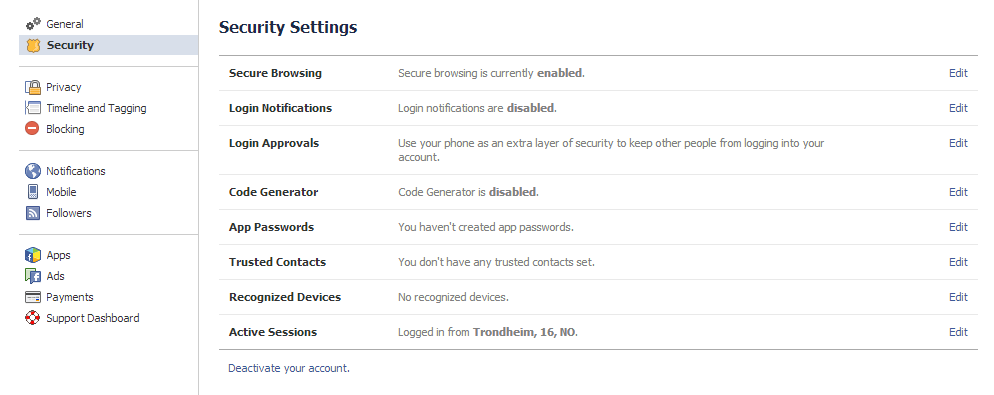
\includegraphics[width=1\textwidth]{default_nov_2013_security.png}
\caption[Default security settings on Facebook November 2013]{\textbf{Default security settings on Facebook November 2013}. This Figure shows the default security settings on Facebook in November 2013.} 
\label{fig:security2013}
\end{figure}

\begin{figure}[h!]
\centering
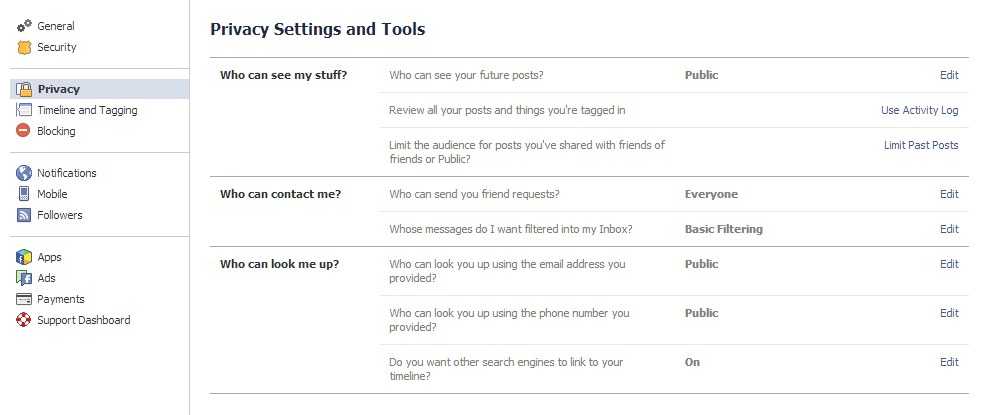
\includegraphics[width=1\textwidth]{default_nov_2013_privacy.png}
\caption[Default privacy settings on Facebook November 2013]{\textbf{Default privacy settings on Facebook November 2013}. This Figure shows the default privacy settings on Facebook in November 2013.} 
\label{fig:privacy2013}
\end{figure}

\begin{figure}[h!]
\centering
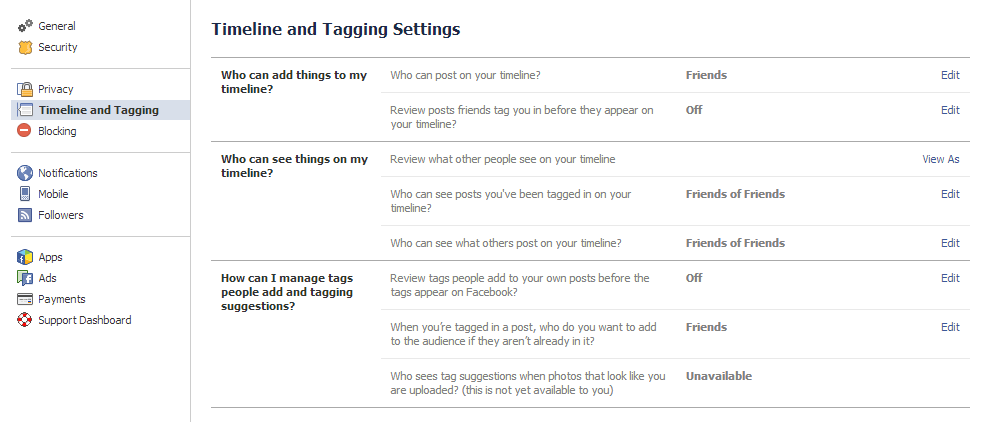
\includegraphics[width=1\textwidth]{default_nov_2013_timelineandtagging.png}
\caption[Default settings for timeline and tagging on Facebook November 2013]{\textbf{Default settings for timeline and tagging on Facebook November 2013}. This Figure shows the default settings for timeline and tagging on Facebook in November 2013.} 
\label{fig:timelineandtagging2013}
\end{figure}

\begin{figure}[h!]
\centering
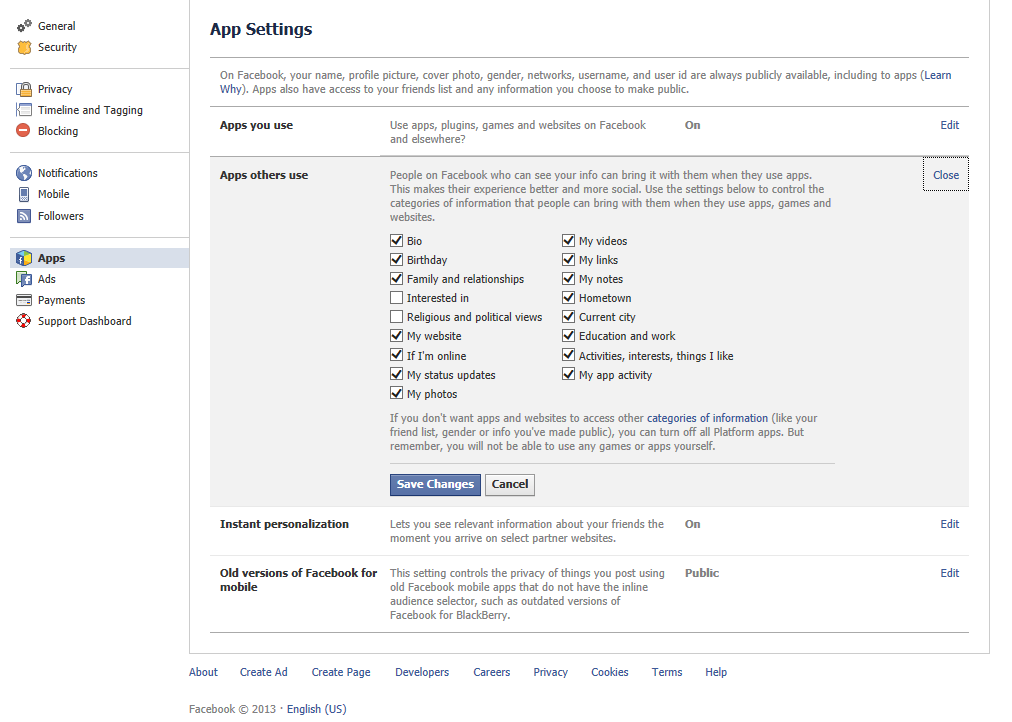
\includegraphics[width=1\textwidth]{default_nov_2013_apps.png}
\caption[Default settings for apps on Facebook November 2013]{\textbf{Default  settings for apps on Facebook November 2013}. This Figure shows the default settings for applications on Facebook in November 2013.} 
\label{fig:apps2013}
\end{figure}

\fref{fig:privacy2013} shows the default privacy settings in November 2013.  \textit{"Who can see your future posts?"} is set to \textit{Public}, which means everyone can view you posts. \textit{"Who can send you friend requests?"} is set to \textit{Everyone}. \textit{"Who can look you up using the email address you provided?"} and \textit{"Who can look you up using the phone number you provided?"} is set to \textit{Public}, which means it is easier for people to find you on Facebook if they know you email or phone number. The setting \textit{"Do you want other search engines to link to your timeline?"} is turned \textit{on}. This means that for example if you google a person, the Facebook profile will appear in the search. To summarize, the privacy settings are \textit{as public as they can get} by default. 

\fref{fig:timelineandtagging2013} shows the default settings for timeline and tagging of Facebook in November 2013. \textit{"Who can post on your timeline?"} is set to \textit{Friends}, which means that only Facebook friends can add things to your timeline. \textit{"Review posts friends tag you in before they appear on your timeline?" }is set to\textit{ off}. This means when friends tags you in something, it will appear on your timeline before you have had a chance to review it. In most cases this is probably fine, but it may occur that a Facebook friends tag you in something you would not prefer to have displayed on your timeline. In these cases it would be desirable to have the review-setting turned on. \textit{"Who can see posts you've been tagged in on your timeline?"} and \textit{"Who can see that others post on your timeline?"} is set to \textit{Friends of Friends}. In contrary to those who can post on your timeline, which are friends, friends of friends are able to view the content added to your timeline. If you have many friends on Facebook, and these friends have many friends each, the audience for posts are suddenly extremely large. 

\paragraph{Default settings does not preserve privacy} It is safe to conclude that the default privacy settings on Facebook anno 2013 is far too public. Unless there are conducted changes to the privacy settings, the timeline will be publicly available, with the exception of posts you've been tagged in and other's posts on your timeline which is "only" visible to friends, and friends of friends. 

\subsection{Default Settings for Teens}

\begin{figure}[h!]
\centering
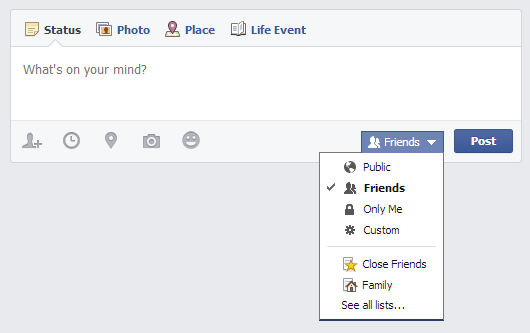
\includegraphics[width=0.8\textwidth]{new_post.png}
\caption[Choosing who can see a status update.]{\textbf{Choosing who can see a status update}. When posting a new post the user can choose the audience the post will be visible to. This can either be "public", "friends", "only me" or "custom".} 
\label{fig:newPost}
\end{figure}

\begin{figure}[h!]
\centering
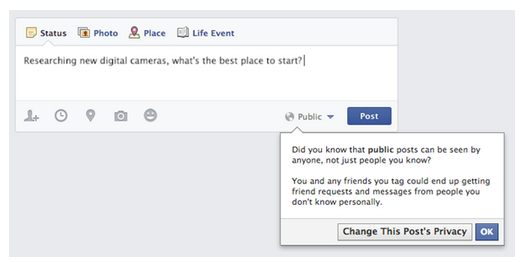
\includegraphics[width=0.8\textwidth]{teensSharePost.png}
\caption[The message shown to teens when posting to the public for the first time]{\textbf{The message shown to teens when posting to the public for the first time.} After the first time they post to the public the message in \fref{fig:sharePost} is shown \cite{defaultTeens}.} 
\label{fig:teensSharePost}
\end{figure}

\begin{figure}[h!]
\centering
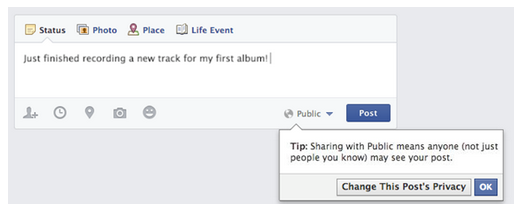
\includegraphics[width=0.8\textwidth]{sharePost.png}
\caption [The message shown to teens when posting to the public, except for the first time]{\textbf{The message shown to teens when posting to the public, except for the first time.} The first time they post to the public the message in \fref{fig:teensSharePost} is shown \cite{defaultTeens}.} 
\label{fig:sharePost}
\end{figure}

Each time a user on Facebook share a status update, the user chooses who the post is visible to, see \fref{fig:newPost}. The change you make will remain the same in future posts, unless you decide to change it. Up until today the default audience is set to "public", but for teens between 13-17 years, it has been "friends of friends". On October 16th Facebook announced to change the default setting for teens \cite{defaultTeens}. Now the initial audience for posts are "friends". Teens can later change this to "public", this was not a option before. Teens are active users of social media, and have want to be heard, either it is political engagement or an opinion on a movie. Further Facebook allows teens to turn on Follow, by doing this their public posts will show up in people's news feeds. Facebook designed these changes to improve the facebook experience for young people. In \cite{defaultTeens} Facebook also makes it clear that they take the safety of teens very seriously, and therefore have created a more extensive warning message, shown in  \fref{fig:teensSharePost}. This message appears when a teen changes the audience for their post. If they continue to post to the public, they will will get an additional reminder message, as shown in  \fref{fig:sharePost}.

\section{Facebook Features - Impact on your Privacy}\label{sec:facebook_features}


\subsection{News Feed}
\paragraph{}
"Somehow we missed this point with News Feed and Mini-Feed and we didn't build in the proper privacy controls right away. This was a big mistake on our part, and I'm sorry for it." \cite{FacebookStoryInceptionToIsp}

\subsection{Facebook Platform - Apps}


\subsection{Beacon}
%-Det må fylles ut mer her!

\paragraph{}
At the end of 2007 Facebook launched the feature called Beacon. Beacon was created to help users easily share information from other websites with their Facebook friends \cite{BeaconWebsites}. Beacon was a key part of the Facebook Ads system. The aim was to connect businesses and users and create a more targeted advertising towards the users. 

When Beacon was launched it had 44 partner site, among these are Live Nation, fandango.com, Trip Advisor, STA travel, eBay, the Knot and Zappos.com. According to the Facebook announcement \cite{BeaconWebsites} these websites could determine which actions was most relevant and appropriate for a user to share on Facebook. This could be anything from watching a video, a new high score on an online game, posting an item for sale or completing a online purchase. When a user, that is logged on to Facebook, enters a website that is part of Beacon, they will receive a message asking whether they would like to share their actions on Facebook. If a users agrees, the users actions on that page will be shown in their news feed or mini feed and shared with their friends.  

Beacon received a lot of attention and privacy concerns. Some websites posted to Facebook without asking the users if they want to share the information first. Beacon is a very short piece of code provided by Facebook. The participating websites implement this code on the actions that they would like people to share. An example described in \cite{beaconMarketsPerspective} is with the blog page TypePad. The user have the opportunity to chose whether Beacon should be turned on or not. When creating a post and publishing it the user receives a small pop-up window in the lower right corner stating that you are now sharing this information with Facebook. The pop-up allow you to answer no, but here you have to be quick, the window is not visible very long. When entering Facebook a message is shown at the top of the users wall. Telling the users that a website have shared information with Facebook. You then have the opportunity to go through and select weather that website is allowed to share at all, to just friends of to the public.  

But not all websites have created an option for the users to themselves choose to opt-in. And pushes to Facebook without notifying the users or lets the users select themselves that they want to share it. An much used example of this is a man buying and engagement ring online and the website posts on Facebook. Before the guy have the time to remove it, both friends and family and also the coming fiancée have seen it. So much for the surprise engagement.  
This is unfortunate for the users, but also for the companies using Beacon, it puts them in a negative light. 

Another problem is that Beacon only checked that a user was logged on Facebook. When several people use one computer it could create problems, since Beacon was machine specific. One family member, the mother, could be logged on while her 10 year old son plays an online game, and manages to make a new high score. This high score will then be posted in the newsfeed on the mothers Facebook profile, and shown to the mothers friends.  Beacon only checks that there is a valid Facebook cookie on the machine and then pushes the content to that Facebook user, without any validation. 

\paragraph{}
In a blog post, Mark Zuckerberg apologized for the way the feature was created and for the handling of the complaints in hindsight. 
\cite{Beacon} 

\subsection{Facebook Connect - "Log in with Facebook"}
From may 2008 users had the ability to connect and log in to other web pages via Facebook, "log in with Facebook" 


\subsection{Timeline}
As mentioned in section \ref{sec:facebookhistory} in Chapter 1, the Facebook timeline was introduced in December 2011 \cite{EvolutionOfFacebook}. This feature made the entire history of the users visible: your posts, posts by others, likes, photos, links, pages liked, comments and other things that you have shared on Facebook. The timeline showed much more than the old profile did, and it was far more visual \cite{timeline}. On the top of your timeline it is room for a big photo. This photo is called a \emph{cover photo}. Cover photos are publicly available, and it is not possible to change the settings for them. You can of course choose which photo you want as your cover photo, or just choose not to have a photo there at all. When scrolling down your timeline , you'll see photos, posts etc. and different events in your life in order of when they happend in time \cite{timeline}. You can look at it as the story of your life. You get the opportunity to "go back in time" and fill in the blanks. If you want to emphasize, for example an event or a photo, you can highlight it with a star, or on the other hand, if you want to hide something from the timeline you can also do so. 

\paragraph{Privacy concerns regarding Facebook timeline}
When timeline was introduced many people became overwhelmed by the changes, and felt they lost control over their privacy. When you agreed to start using timeline, you got a certain period of time to review and edit your timeline before making it public. This gave the users the opportunity to clean up their timeline before everyone else could view the content of it. Cleaning up the timeline can be done using something called the "Activity Log" \cite{activitylog}, which is shown in \fref{fig:activitylog}. The activity log is basically a list over everything ever done in connection with you on Facebook, either done by you or by others. The activity log also makes it easy to view and change the audience for the different "activities". If you are an active user of Facebook, reviewing the whole activity log can be very time consuming. 

\begin{figure}[h!]
\centering
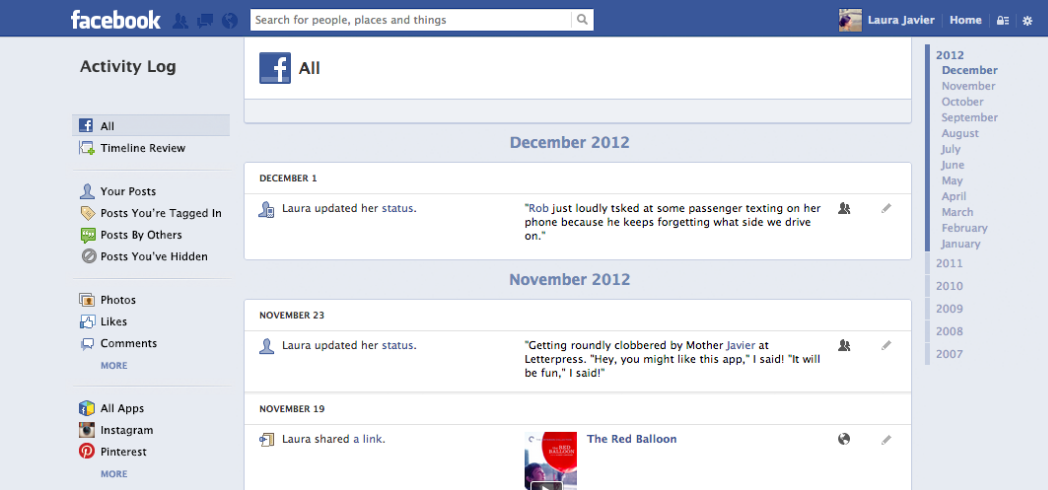
\includegraphics[width=1\textwidth]{activity_log.png}
\caption [Example of an activity log on Facebook.]{\textbf{Example of an activity log on Facebook}. On the left side you see types of content. If you want to view for example "Posts by others" you can do so by clicking on it. To the right you see a list of the years and months. You can click on which year or month you want, and review the activity from that year/month \cite{activitylog}} 
\label{fig:activitylog}
\end{figure}

\paragraph{}
The introduction of timeline was not in itself a privacy breach since you had, and still have, the opportunity to decide what you want to be visible on it, and what you want to hide. On the other hand, there are people who are extra exposed when Facebook introduced new major changes, like the timeline. Lets refer back to section \ref{sec:relatedwork_facebookprivacy} in Chapter \ref{chp:relatedwork}, where we highlighted some of the findings from the survey addressed in the paper "Facebook privacy settings; Who cares?" by danah boyd and Eszter Hargittai \cite{whocares}. boyd and Hargittai concluded their paper, based on their survey and findings, that experience and Internet skill is important to take into account in regard to how people handle their privacy settings on Facebook. Since familiarity with technology plays a role in how people handle their Facebook privacy settings, one can assume that the least skilled people get more exposed when Facebook changes the outline of the default privacy settings. 
This can be seen in the context with the introduction of the timeline. The least skilled users of Facebook that perhaps do not know how to change their privacy settings, probably was left extra exposed when the timeline was introduced and their timeline may have shown, and may still show, more than they actually would prefer. 

There also exits privacy settings connected to you timeline under "Timeline and tagging" in your settings on Facebook. You can regulate who can add things to your timeline, and who can see things on your timeline. Under "Privacy" you can also regulate who can see your future posts. 

\subsection{Graph Search}


\subsection{Facebook Removes Search Privacy Setting}
Facebook announced October 11 that they will remove the setting that has made it possible for Facebooks users to hide from the ability to be looked up on the Internet\cite{searchSetting}. It was only the users that have not used the setting "who can look up my timeline by name" in December by last year that was affected by the change. Facebook explains the removal of the feature by it being outdated, and that there are several others ways to find a persons time line. They argue that it can be confusing for the user when they try to look up someone and do not find them. Mark Zuckerberg said that a users should do things they want to keep secret.

(sånn jeg ser det så er det jo fult mulig å søke opp hvem som helt på faceboko sin egen søkefunksjon, det betyr jo ikke ta jeg ønsker å være søkbar på google. 


\section{Zuckerberg's Thoughts}

\paragraph{}
Zuckerberg ones said this about Facebook in a one of his meetings: "I mean, one way to look at the goal of the site is to increase people’s understanding of the world around them, to increase their information supply," he said. "The way you do that best is by having people share as much information as they are comfortable with. The way you make people comfortable is by giving them control over exactly who can see what" \cite{MeMedia}.

\paragraph{}
This comment from Zuckerberg brings out his thoughts around the privacy issues. He wants the users of Facebook to be comfortable with sharing information, and give them this confidence by giving them control. In general the privacy settings and restrictions that Facebook has have protected the users. They can easily change the setting and decide who can see what. Zuckerburg firmly means that you should not post comments or pictures of things you do not want anybody else to see. And if a user does so, the user has to take the blame for it, not Facebook. Zuckerberg was once asked about pictures put on Facebook of students drinking at an East Coast college, which led to some students being expelled. His answer to this question was: "First of all, it's pretty stupid if you put up pictures of you doing drugs on Facebook. I think that that's just sort of the deviant behavior on the very far end of the distribution. I bet that those kids do not post pictures of them doing drugs on Facebook anymore." He added that he meant this was a "pretty shitty way to learn that" \cite{MeMedia}.

\paragraph{}






\paragraph{}
Mark Zuckerberg wrote this in a letter to possible investors \cite{LetterToInvestors};

\textit{Facebook was not originally created to be a company. It was built to accomplish a social mission - to make the world more open and connected.}

\textit{People sharing more - even if just with their close friends or families - creates a more open culture and leads to a better understanding of the lives and perspectives of others. We believe that this creates a greater number of stronger relationships between people, and that it helps people get exposed to a greater number of diverse perspectives.}

\textit{By helping people form these connections, we hope to rewire the way people spread and consume information. We think the world's information infrastructure should resemble the social graph - a network built from the bottom up or peer-to-peer, rather than the monolithic, top-down structure that has existed to date. We also believe that giving people control over what they share is a fundamental principle of this rewiring.}

\textit{We think a more open and connected world will help create a stronger economy with more authentic businesses that build better products and services.}

\paragraph{Skal vi ha med det her?}
User control became a hot topic already in 2006. There had been reported that sex- offenders was using social networks to pick out their victims. MySpace found out that several teenagers had been assaulted by people they meet at their web page. Facebook also received some negative mention in the press. Numerous times the campus police had to shut down big parties announced on Facebook. In 2005 a student a Fisher college was expelled after posting this comment about the schools police officer "needs to be eliminated" \cite{MeMedia}.
